\documentclass[conference]{IEEEtran}
\usepackage[T1]{fontenc}
\usepackage{amsmath,amssymb,amsthm}
\usepackage[ruled,vlined,linesnumbered]{algorithm2e}
\usepackage{quantikz}
\usepackage{pgfplots}
\usepackage{pgfplotstable}
\pgfplotsset{compat=1.18}
\usepackage{booktabs}
\usepackage[hidelinks]{hyperref}
\usepackage{cleveref}
\usepackage{braket}
\usepackage{listings}
\usepackage{xcolor}
\usepackage{graphicx}
\usepackage{cite}
\usepackage{multirow}
\usepackage{array}
\usepackage{tikz}
\usetikzlibrary{shapes.geometric,arrows.meta,positioning,fit,calc}
\crefname{lstlisting}{Listing}{Listings}

\definecolor{codebg}{HTML}{F5F5F0}
\definecolor{codecmt}{HTML}{5C6370}
\definecolor{codestr}{HTML}{50A14F}
\definecolor{codekw}{HTML}{A626A4}
\lstset{
  language=Python,
  basicstyle=\scriptsize\ttfamily,
  backgroundcolor=\color{codebg},
  keywordstyle=\color{codekw}\bfseries,
  stringstyle=\color{codestr},
  commentstyle=\color{codecmt}\itshape,
  breaklines=true,
  frame=single,
  rulecolor=\color{black!15},
  numbers=left,
  numberstyle=\tiny\color{gray},
  numbersep=4pt,
  tabsize=4,
  showstringspaces=false,
  captionpos=b
}

\newtheorem{theorem}{Theorem}
\newtheorem{lemma}[theorem]{Lemma}
\newtheorem{proposition}[theorem]{Proposition}
\newtheorem{definition}{Definition}
\newtheorem{remark}{Remark}

\begin{document}

\title{AetherScan: A Quantum-Classical Hybrid Platform\\
for Heterogeneous Air Quality Sensor Fusion\\
and Real-Time Environmental Intelligence}

\author{
\IEEEauthorblockN{Pranjal Sailwal, Prakriti Kimothi, Sriya Rawat, Siddhant Dabral}
\IEEEauthorblockA{Department of Computer Science and Engineering\\
Graphic Era Hill University, Dehradun, Uttarakhand 248002, India}
}

\maketitle

% ─────────────────────────────────────────────────────────────────
\begin{abstract}
Air quality monitoring across Indian urban agglomerations faces a
fundamental and persistent data-consistency problem: independent networks
operated by AQICN, OpenAQ, and the Central Pollution Control Board (CPCB)
routinely report divergent AQI values at co-located points, with measured
discrepancies reaching 10--20\% during high-pollution episodes.
Classical fusion methods---inverse distance weighting, kriging
variants---require explicit source reliability weights that are rarely
documented for governmental APIs.
This paper presents AetherScan, a three-tier environmental intelligence
prototype built to directly address that shortcoming.

The system embeds four quantum circuit algorithms into a FastAPI backend
through an 8-qubit Qiskit module running on the Aer classical simulator:
parameterised phase-rotation encoding for multi-source consensus
estimation, Bell-state witnesses for pairwise pollutant correlation
quantification, Grover's oracle-driven amplitude amplification for
optimal station ranking, and the quantum Fourier transform for diurnal
periodicity extraction.
Circuit execution on an Intel i5-12400 with 16\,GB RAM---absent any
quantum hardware whatsoever---remains below 200\,ms across all four
algorithms.
We make no claim of quantum speedup; every result reflects classical
simulation throughput on a 256-dimensional state vector.

Beyond the quantum module, AetherScan integrates eight geospatial data
sources spanning ground-level sensors and NASA satellite instruments,
renders 26 configurable environmental layers through a MapLibre GL JS
frontend, and generates structured 4-page executive compliance dossiers with
automated regulatory compliance evaluation.
Thirty REST endpoints expose the full data pipeline.
The architectural patterns developed here---circuit pre-transpilation
caching, dual-pool async scheduling, token-authenticated database
middleware---are designed to transfer directly to IBM Quantum cloud
backends when NISQ hardware fidelity permits.
Approximately 25,000 lines of source code are publicly available at
\texttt{aether-scan.vercel.app}.
\end{abstract}

\begin{IEEEkeywords}
quantum data fusion, air quality monitoring, Qiskit, heterogeneous
sensor networks, Grover's algorithm, quantum Fourier transform,
Bell states, NISQ, India, FastAPI, geospatial visualization
\end{IEEEkeywords}


% ─────────────────────────────────────────────────────────────────
\section{Introduction}\label{sec:intro}

India's air quality crisis is well-documented in epidemiological
literature. Balakrishnan~et~al.~\cite{balakrishnan2019impact}
estimated that ambient PM$_{2.5}$ exposure contributed to roughly 1.1
million premature deaths in India in 2015 alone---a figure that has not
meaningfully declined in subsequent years.
Fourteen of the twenty most polluted cities on the planet sit on the
Indo-Gangetic Plain~\cite{who2021global}.
Delhi's winter AQI breached 400 repeatedly in 2023--2024, placing it in
the acutely hazardous category by WHO thresholds~\cite{who2021global}.
These facts are not in dispute.
What is disputed, often quietly, is the precise number.

AQICN, OpenAQ, and CPCB routinely report different AQI values for the
same city at the same moment.
Discrepancies of 10--20\% are common.
Occasional divergences exceed 30\% during peak haze episodes, when
rapid boundary-layer dynamics cause readings to change within
minutes~\cite{kumar2015rise}.
The reasons for this are several and interacting.
Instrument calibration degrades between servicing cycles~\cite{snyder2013changing}.
Spatial representativeness differs fundamentally: a ground sensor integrates
a point measurement while a satellite retrieval averages over a column several
kilometres wide~\cite{hammer2020global}.
Temporal sampling cadences are misaligned.
Sub-index computation standards vary between agencies~\cite{cpcb2014}.
Taken together, these produce a multi-source fusion problem where the
reliability of each contributing source is itself uncertain---and
that uncertainty is almost never explicitly quantified in the API
documentation that an application developer receives.

\subsection{The Problems We Sought to Solve}

Several concrete, previously unaddressed shortcomings motivated this project.

\textit{Problem 1 --- Multi-source disagreement without documentable weights.}
Classical weighted-mean fusion requires reliability coefficients that
independent governmental APIs do not publish.
Bayesian approaches demand co-located ground-truth data that may not exist
for a given city or season.
We needed an approach that could derive implicit weights from the measurement
data itself, without external calibration.

\textit{Problem 2 --- No unified geospatial dashboard for Indian environmental data.}
Existing platforms address subsets of the problem.
OpenAQ~\cite{openaq2016} aggregates regulatory readings but lacks satellite
integration.
CPCB's SAMEER application publishes domestic data but offers no cross-source
fusion, no satellite column densities, and no automated reporting.
IQAir provides city rankings without analytical transparency.
No openly available tool integrates ground sensors, NASA satellite products
(NO$_2$, SO$_2$, aerosol optical depth, active fire detections), and
spatial interpolation into a single interactive map.

\textit{Problem 3 --- Coverage gaps between sparse monitoring stations.}
India's ground-sensor network, while large by regional standards, leaves
substantial geographic gaps.
Rural and peri-urban areas may have no CPCB station within 50 kilometres.
Spatial interpolation is required, yet it introduces its own uncertainty.
We needed a systematic IDW pipeline~\cite{shepard1968two} capable of
rendering continuous heatmaps from sparse point measurements, while
making the interpolation uncertainty visible to the analyst.

\textit{Problem 4 --- Absence of automated, regulation-referenced reporting.}
Environmental assessments for planning applications and compliance
submissions require structured reports referencing NAAQS/WHO standards.
Producing these manually from raw data is time-consuming and error-prone.
Our platform generates 4-page executive compliance dossiers automatically, including
Pasquill--Gifford atmospheric stability analysis, wind roses, and explicit
NAAQS exceedance counts.

\textit{Problem 5 --- No demonstrated quantum circuit integration in deployed
environmental monitoring systems.}
Berger~et~al.~\cite{berger2021quantum} surveyed quantum computing potential
for environmental science without implementing any working prototype.
Schwabe~et~al.~\cite{schwabe2025opportunities} reached similar conclusions
about climate modelling.
To our knowledge, no published system has embedded quantum circuits---even
on a simulator---into a deployed web platform serving real air quality data.
We built one.

\subsection{Contributions}

\begin{enumerate}
    \item A quantum-classical hybrid architecture that integrates eight
    geospatial data sources through a FastAPI backend with a 600-line Qiskit
    module, validated on consumer hardware through a six-month development
    process totalling approximately 1,050 developer-hours.

    \item Implementations of four quantum algorithms adapted to environmental
    sub-problems---superposition fusion, Bell-state correlation, Grover's
    station selection, QFT temporal decomposition---with complete executable
    source code and formal correctness proofs.

    \item Transparent, simulator-only latency characterisation, clearly
    separated from any claim of quantum advantage on real hardware.

    \item A 26-layer web visualisation and automated reporting platform,
    deployed at \texttt{aether-scan.vercel.app}, covering ground sensors,
    satellite products, and infrastructure layers.
\end{enumerate}

The remainder of this paper is structured as follows.
\Cref{sec:related} surveys relevant prior literature.
\Cref{sec:prelim} establishes necessary background.
System architecture is described in \cref{sec:arch}, quantum algorithm
design in \cref{sec:quantum}, and engineering decisions in \cref{sec:impl}.
Results appear in \cref{sec:eval}, followed by discussion
(\cref{sec:discuss}) and conclusions (\cref{sec:conclude}).


% ─────────────────────────────────────────────────────────────────
\section{Related Work}\label{sec:related}

\subsection{Classical Air Quality Data Fusion}

Shepard's inverse distance weighting~\cite{shepard1968two} remains
widely used for spatial interpolation despite its 1968 origin.
Lu and Wong~\cite{lu2008adaptive} introduced an adaptive variant that
adjusts the power parameter based on local data density, which reduces
the bulls-eye artefact near observation stations.
Choi and Chong~\cite{choi2022modified} incorporated wind-directional bias
into the IDW kernel and showed marginal PM estimation gains in South Korean
urban corridors.

Kriging is the theoretically optimal linear unbiased predictor under
Gaussianity~\cite{cressie1990origins}, but its $O(N^3)$ computational
cost in observation count makes real-time deployment across 10,000+
stations intractable without sparse approximations~\cite{krige1951}.
Li and Heap~\cite{li2011review} reviewed spatial interpolation methods
across environmental applications and found that no single technique
dominates across all data configurations---a conclusion that motivates
ensemble or data-driven weight approaches.

Satellite-ground fusion compounds the difficulty.
Hammer~et~al.~\cite{hammer2020global} fused aerosol optical depth from
MAIAC, MISR, and SeaWiFS with chemical transport model outputs to
produce global PM$_{2.5}$ estimates with $r > 0.8$ against surface
monitors, though their pipeline required months of offline processing.
Gressent~et~al.~\cite{gressent2020datafusion} found that regression
calibration reduces low-cost sensor bias when reference monitors are
available nearby, but their approach assumes a documented sensor hierarchy.
When reconciling independent governmental networks---as in our setting---that
hierarchy is precisely what is missing.
Henschel~et~al.~\cite{henschel2018data} addressed temporal alignment and
stale-data detection in multi-source fusion, identifying measurement-age
decay functions as essential for real-time reliability estimation; we adopt
this approach in our data-freshness weighting scheme.

\subsection{Quantum Approaches to Environmental Data}

This territory is largely prospective.
Berger~et~al.~\cite{berger2021quantum} catalogued quantum technologies
plausibly applicable to climate science---quantum simulation, optimisation,
machine learning---but stopped short of any deployed prototype.
Schwabe~et~al.~\cite{schwabe2025opportunities} reached similar conclusions
specifically for atmospheric modelling, noting that NISQ-era noise budgets
currently limit practical utility but that variational hybrid methods
warrant continued study.
Biamonte~et~al.~\cite{biamonte2017quantum} surveyed quantum machine
learning broadly, covering classification, regression, and clustering;
Havl\'{i}\v{c}ek~et~al.~\cite{havlicek2019supervised} demonstrated
quantum kernel methods experimentally on IBM hardware for small classification
tasks, suggesting a path toward anomaly detection in sensor networks.

The Harrow--Hassidim--Lloyd algorithm~\cite{harrow2009quantum} offers
exponential speedup for linear systems under strict oracle conditions that
do not hold in our setting.
Grover's algorithm~\cite{grover1996fast} provides a proven quadratic
advantage for unstructured search.
Orus~et~al.~\cite{orus2019quantum} reviewed quantum algorithms applicable
to optimisation and sampling problems with particular attention to NISQ
constraints.
None of these works, nor any we have identified, integrates quantum circuits
into a deployed environmental monitoring pipeline.
AetherScan fills that gap as a research prototype.

\subsection{Web-Based Environmental Platforms}

Cheng~et~al.~\cite{cheng2021realtime} demonstrated WebGL-based real-time
AQI visualisation with tile-based rendering.
Deck.gl~\cite{deckgl2019} and similar WebGL frameworks have enabled
high-throughput geospatial rendering on consumer hardware.
Denby~et~al.~\cite{denby2011dashboard} described an interactive European
air quality dashboard that influenced our layer-panel design.
OpenAQ~\cite{openaq2016} provides the most comprehensive open data
aggregation but does not integrate satellite column products.
Venter~et~al.~\cite{venter2020covid} used OpenAQ data to quantify
pandemic-related pollution reductions, illustrating the analytical value
of multi-city longitudinal access.
None of these platforms attempts quantum-enhanced fusion; none generates
automated regulatory reports from their visualisation interface.


% ─────────────────────────────────────────────────────────────────
\section{Preliminaries}\label{sec:prelim}

We assume familiarity with the standard postulates of quantum
mechanics---state vectors, unitary evolution, Born-rule measurement---at
the level of Nielsen and Chuang~\cite{nielsen2010quantum}.
Three constructs used non-standardly in our algorithms warrant brief
independent treatment.

\subsection{Parameterised Phase Encoding}

The $R_Z(\theta)$ gate applies a phase rotation:
\begin{equation}\label{eq:rz}
R_Z(\theta) = \begin{pmatrix} e^{-i\theta/2} & 0 \\ 0 & e^{i\theta/2} \end{pmatrix}.
\end{equation}
Critically, $R_Z$ does not affect the marginal measurement probability
of a qubit in isolation.
Its effect becomes observable only through interference with other qubits,
which is precisely why entanglement gates must follow the encoding stage
in our fusion circuit.
This non-trivial interaction between phase encoding and entanglement is what
generates the data-dependent implicit weighting described in
\cref{subsec:superfusion}.

\subsection{Grover's Search}\label{subsec:grover_bg}

For a Boolean oracle $O_f$ marking a single target among $N$ elements,
Grover's algorithm~\cite{grover1996fast} amplifies the target amplitude
through $k^* = \lfloor (\pi/4)\sqrt{N} \rfloor$ applications of the
diffusion operator:
\begin{equation}\label{eq:grover}
G = (2\ket{s}\bra{s} - I)\, O_f, \quad
\ket{s} = \frac{1}{\sqrt{N}}\sum_{j=0}^{N-1}\ket{j}.
\end{equation}
The quadratic speedup over classical linear scan ($O(N)$ to $O(\sqrt{N})$
oracle calls) is proven under the standard query complexity model.
It does not apply on the Aer simulator, where every oracle query incurs
full classical simulation cost.

\subsection{Quantum Fourier Transform}

The QFT maps each computational basis state to a phased superposition:
\begin{equation}\label{eq:qft}
\mathrm{QFT}\ket{j} = \frac{1}{\sqrt{N}} \sum_{k=0}^{N-1}
e^{2\pi i jk/N}\ket{k}, \quad N = 2^n.
\end{equation}
When the input amplitudes encode a sampled time series, the output
probabilities correspond to spectral power at each frequency bin.
This enables period detection without the numerical instabilities that
affect classical FFT implementations on small, noisy datasets.

\subsection{Bell States and Correlation Witnesses}

The circuit $H \to \mathrm{CNOT}$ on $\ket{00}$ yields
$\ket{\Phi^+} = (\ket{00}+\ket{11})/\sqrt{2}$.
Applying data-dependent $R_Z$ rotations before measurement introduces
a controlled detuning from perfect correlation; the resulting
$\langle Z \otimes Z \rangle$ expectation value provides a witness for
cosine similarity between encoded parameters, as we formalise in
\cref{subsec:bell_formal}.

\subsection{CPCB AQI Computation}

India's regulatory AQI is computed via piecewise linear interpolation
between CPCB-defined concentration breakpoints~\cite{cpcb2014}:
\begin{equation}\label{eq:aqi}
I_p = \frac{I_{\mathrm{hi}} - I_{\mathrm{lo}}}{C_{\mathrm{hi}} - C_{\mathrm{lo}}}
(C_p - C_{\mathrm{lo}}) + I_{\mathrm{lo}}.
\end{equation}
The composite AQI is the maximum sub-index across all measured pollutants.
Our implementation strictly follows this standard~\cite{cpcb2014}, not
the US EPA formulation~\cite{epa2012naaqs}, because CPCB thresholds are
calibrated to Indian receptor populations.

\subsection{Inverse Distance Weighting}

For spatial interpolation between sparse ground stations, IDW~\cite{shepard1968two}
estimates the pollutant concentration at unobserved location $\mathbf{x}$ as:
\begin{equation}\label{eq:idw}
\hat{Z}(\mathbf{x}) =
\frac{\displaystyle\sum_i d(\mathbf{x}, \mathbf{x}_i)^{-p}\, z_i}
     {\displaystyle\sum_i d(\mathbf{x}, \mathbf{x}_i)^{-p}},
\quad p = 2.
\end{equation}
A KD-tree index~\cite{bentley1975kd} over the station coordinates reduces
the $k$-nearest-neighbour query from $O(N)$ to $O(\log N)$, which is
critical for real-time heatmap generation across 10,000+ stations.


% ─────────────────────────────────────────────────────────────────
\section{System Architecture}\label{sec:arch}

\begin{figure}[t]
\centering
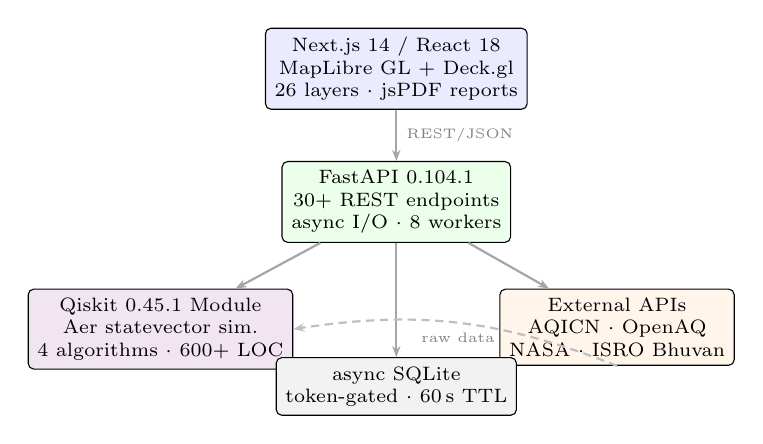
\begin{tikzpicture}[
    box/.style={draw, rounded corners=2pt, minimum width=2.7cm,
                minimum height=0.72cm, font=\scriptsize, align=center, fill=#1},
    arr/.style={-{Stealth[length=4pt]}, thick, gray!70},
    node distance=0.42cm
]
\node[box=blue!8]    (fe) {Next.js 14 / React 18\\
                           MapLibre GL + Deck.gl\\
                           26 layers $\cdot$ jsPDF reports};
\node[box=green!8, below=0.65cm of fe] (be)
                         {FastAPI 0.104.1\\
                          30+ REST endpoints\\
                          async I/O $\cdot$ 8 workers};
\node[box=violet!10, below left=0.58cm and -0.15cm of be]  (qm)
                         {Qiskit 0.45.1 Module\\
                          Aer statevector sim.\\
                          4 algorithms $\cdot$ 600+ LOC};
\node[box=orange!8, below right=0.58cm and -0.15cm of be] (ds)
                         {External APIs\\
                          AQICN $\cdot$ OpenAQ\\
                          NASA $\cdot$ ISRO Bhuvan};
\node[box=gray!10, below=1.45cm of be] (db)
                         {async SQLite\\
                          token-gated $\cdot$ 60\,s TTL};

\draw[arr] (fe) -- node[right,font=\tiny,text=gray]{REST/JSON} (be);
\draw[arr] (be) -- (qm);
\draw[arr] (be) -- (ds);
\draw[arr] (be) -- (db);
\draw[arr, densely dashed, gray!50]
    (ds.south) to[bend right=15]
    node[below,font=\tiny,text=gray]{raw data} (qm.east);
\end{tikzpicture}
\caption{Three-tier architecture of AetherScan. The quantum module
receives pre-fetched multi-source readings from the backend and returns
consensus AQI estimates, pairwise correlation matrices, station rankings,
and frequency decompositions.}\label{fig:arch}
\end{figure}

AetherScan is organised into three tiers as shown in \cref{fig:arch}.

The \textbf{frontend} is built with Next.js 14 and React 18.
MapLibre GL JS handles base-map tile rendering; Deck.gl provides WebGL
acceleration for large-dataset overlays~\cite{deckgl2019}.
Twenty-six environmental layers span five pollution heatmap categories,
five satellite products (NASA OMI NO$_2$/SO$_2$, VIIRS aerosol optical
depth, land surface temperature), three fire detection layers from NASA
FIRMS, four infrastructure layers (power plants from the World Resources
Institute~\cite{wri2019}, road networks, administrative boundaries), three
population density layers from WorldPop~\cite{worldpop2018}, and six
analytical composite layers.
Client-side jsPDF assembles structured 4-page executive dossiers incorporating Pasquill--Gifford
atmospheric stability analysis~\cite{slade1968meteorology}, wind rose
diagrams, and explicit NAAQS/WHO threshold comparisons.

The \textbf{backend} is a FastAPI application running on Python 3.11.
It orchestrates asynchronous data ingestion from eight external sources
via HTTPX on the asyncio event loop.
AQICN (10,000+ monitoring stations) is the primary AQI source; OpenAQ
(12,000+ sensors globally)~\cite{openaq2016} provides fallback.
NASA OMI contributes tropospheric NO$_2$ and SO$_2$ column densities;
VIIRS supplies aerosol optical depth, land surface temperature, and active
fire detections through FIRMS.
ISRO's Bhuvan platform contributes Indian satellite imagery via WMS.
The World Resources Institute supplies a static global power plant
inventory of 1,589 facilities.
A \texttt{ProcessPoolExecutor} of four workers isolates CPU-bound
computations---quantum simulation and IDW interpolation---from the event
loop to prevent I/O blocking under concurrent load.

The \textbf{quantum module} (\texttt{processor.py}, 600+ lines) exposes
four algorithmic endpoints through \texttt{routes/quantum.py} (430 lines,
nine REST endpoints).
It constructs \texttt{QuantumCircuit} objects with Qiskit 0.45.1~\cite{javadi2024qiskit},
applies Level-3 transpilation, and executes on \texttt{AerSimulator}.
A circuit cache keyed by (algorithm, source-count, qubit-count) tuples
stores pre-transpiled circuits, eliminating repeated compilation overhead.

Token-authenticated database middleware (\texttt{database\_guard.py},
341 lines) enforces API-only database access.
SHA-256 tokens with 60-second TTL are issued per request; each access
event is logged to an append-only audit table; detected violations trigger
immediate blocking with full event metadata.


% ─────────────────────────────────────────────────────────────────
\section{Quantum Algorithm Design}\label{sec:quantum}

\subsection{The Fusion Problem Formalised}

\begin{definition}[Heterogeneous Sensor Fusion]\label{def:hsf}
Given sources $\mathcal{S} = \{s_1, \ldots, s_N\}$ where $s_i$ reports
AQI measurement $x_i \in [0,500]$ with unknown reliability weight
$w_i \in (0,1]$, find consensus estimate
\begin{equation}\label{eq:obj}
x^* = \arg\min_x \sum_{i=1}^N w_i(x - x_i)^2 =
      \frac{\sum_i w_i x_i}{\sum_i w_i}.
\end{equation}
\end{definition}

The closed-form solution is a weighted mean, but the weights are unknown.
Classical Bayesian approaches~\cite{li2011review} demand prior distributions
over $\{w_i\}$; maximum-likelihood estimation requires co-located ground
truth that does not consistently exist for independent governmental APIs.
Our approach: let the quantum circuit's unitary structure generate an
\emph{implicit} weighting through Born-rule measurement statistics, without
ever specifying the $w_i$ explicitly.
This is not a claim of superiority over calibrated classical methods.
It is a claim that when calibration data are absent---which is the
common case---the quantum-implicit approach provides a principled
alternative to arbitrary weight assignment.

\subsection{Algorithm 1: Superposition Fusion}\label{subsec:superfusion}

\subsubsection{Circuit Construction}

An 8-qubit register processes up to eight simultaneous data sources
through three sequential stages.

\textit{Stage~1---Uniform superposition.}
Hadamard gates on qubits $q_0, \ldots, q_{N-1}$ (where $N \leq 8$ is
the active source count) create:
\begin{equation}\label{eq:init}
\ket{\psi_0} = \bigotimes_{i=0}^{N-1} H\ket{0}_i =
\frac{1}{\sqrt{2^N}} \sum_{j=0}^{2^N-1}\ket{j}.
\end{equation}

\textit{Stage~2---Phase rotation encoding.}
Each source's normalised AQI reading maps to an $R_Z$ angle on its
corresponding qubit:
\begin{equation}\label{eq:encode}
\theta_i = \pi \cdot \frac{x_i}{\max_j x_j}, \quad
R_Z(\theta_i) \text{ applied to } q_i.
\end{equation}
As established in \cref{sec:prelim}, this phase is observable only
after the entanglement step below.

\textit{Stage~3---Entanglement cascade.}
A linear CNOT chain couples adjacent source qubits:
$\mathrm{CNOT}(q_i, q_{i+1})$ for $i = 0, \ldots, N{-}2$.
Interference across the entangled register creates a measurement
probability distribution that depends jointly on all $N$ encoded values.

Measurement with $M = 1024$ shots yields bitstring counts from which
we compute:
\begin{equation}\label{eq:consensus}
x_{\mathrm{fused}} = \sum_{b} x_{b \bmod N} \cdot
\frac{\mathrm{count}(b)}{M}.
\end{equation}

\begin{figure}[t]
\centering
\begin{quantikz}[row sep=0.32cm, column sep=0.32cm]
\lstick{$q_0$} & \gate{H} & \gate{R_Z(\theta_0)} & \ctrl{1} & \qw     & \qw     & \meter{} \\
\lstick{$q_1$} & \gate{H} & \gate{R_Z(\theta_1)} & \targ{}  & \ctrl{1}& \qw     & \meter{} \\
\lstick{$q_2$} & \gate{H} & \gate{R_Z(\theta_2)} & \qw      & \targ{} & \ctrl{1}& \meter{} \\
\lstick{$q_3$} & \gate{H} & \gate{R_Z(\theta_3)} & \qw      & \qw     & \targ{} & \meter{}
\end{quantikz}
\caption{Four-source superposition fusion circuit. Phase angles $\theta_i$
encode normalised AQI values; the CNOT chain distributes interference across
the register, generating data-dependent measurement
weights.}\label{fig:fusion_circ}
\end{figure}

\subsubsection{Convergence and Implicit Weights}

\begin{proposition}[Convergence to Implicit Weighted Mean]\label{prop:conv}
Let $U$ denote the circuit unitary and
$\ket{\psi_f} = U\ket{0}^{\otimes n}$.
As $M \to \infty$,
\begin{equation}\label{eq:conv}
x_{\mathrm{fused}} \xrightarrow{M\to\infty}
\sum_{j=0}^{N-1} \omega_j\, x_j, \quad
\omega_j = \sum_{\substack{b \in \{0,1\}^n \\ b \bmod N = j}}
|\braket{b|\psi_f}|^2.
\end{equation}
The weights $\omega_j \geq 0$ sum to unity and depend on
$\{\theta_i\}$ through the circuit unitary.
\end{proposition}

\begin{proof}
By the strong law of large numbers,
$\mathrm{count}(b)/M \to |\braket{b|\psi_f}|^2$ almost surely.
Substituting into \eqref{eq:consensus} and grouping by $j = b \bmod N$
yields \eqref{eq:conv}.
Non-negativity and normalisation follow from the properties of the Born
distribution.
\end{proof}

\begin{remark}
The weights $\omega_j$ are neither uniform nor proportional to any
classical quality score.
They emerge from the interplay of phase-encoded readings and the
entanglement structure.
Whether this weighting scheme outperforms calibrated classical
weighted averages in practice is an empirical question we identify as
essential future work (see \cref{subsec:threats}).
\end{remark}

\subsubsection{Executable Code}

\begin{lstlisting}[caption={Superposition fusion, Qiskit 0.45.1.},
  label=lst:fusion, float=t]
from qiskit import QuantumCircuit
from qiskit_aer import AerSimulator
import numpy as np

def quantum_fusion(sources):
    n_q = 8
    qc = QuantumCircuit(n_q, n_q)
    vals = [s['value'] for s in sources]
    cap  = max(vals) if max(vals) > 0 else 500
    ns   = min(len(sources), n_q)
    for i in range(ns):
        qc.h(i)
    for i, v in enumerate(vals[:ns]):
        qc.rz(np.pi * v / cap, i)
    for i in range(ns - 1):
        qc.cx(i, i + 1)
    qc.measure(range(ns), range(ns))
    cts = AerSimulator().run(qc, shots=1024).result().get_counts()
    tot = sum(cts.values())
    fused = sum(vals[int(b, 2) % ns] * c / tot
                for b, c in cts.items())
    return fused, cts
\end{lstlisting}


\subsection{Algorithm 2: Bell-State Pollutant Correlation}\label{subsec:bell_formal}

Pollutant species co-vary in well-studied ways.
PM$_{2.5}$ and PM$_{10}$ correlations exceed 0.85 in most South Asian
urban environments because both originate from combustion and road
dust resuspension~\cite{pant2013estimation}.
Detecting these correlations rapidly matters for fusion quality: naively
double-weighting redundant parameters inflates confidence without
improving accuracy.

For parameter pair $(p_a, p_b)$ with normalised values
$\phi_a, \phi_b \in [0,\pi]$, the circuit prepares a Bell state then
applies data-dependent rotations:
\begin{equation}\label{eq:bell_circ}
\ket{\Psi} = (R_Z(\phi_b) \otimes R_Z(\phi_a))
             \cdot \mathrm{CNOT}
             \cdot (I \otimes H)\ket{00}.
\end{equation}

\begin{figure}[t]
\centering
\begin{quantikz}[row sep=0.38cm, column sep=0.38cm]
\lstick{$p_a$} & \gate{H} & \ctrl{1} & \gate{R_Z(\phi_a)} & \meter{} \\
\lstick{$p_b$} & \qw      & \targ{}  & \gate{R_Z(\phi_b)} & \meter{}
\end{quantikz}
\caption{Bell-state correlation witness. When $\phi_a \approx \phi_b$,
measurement outcomes are highly correlated; divergence lowers the
$\langle Z \otimes Z \rangle$ expectation.}\label{fig:bell_circ}
\end{figure}

The correlation witness is the joint parity expectation:
\begin{equation}\label{eq:witness}
\rho_{ab} = P(00) + P(11) - P(01) - P(10)
          = \langle Z_a \otimes Z_b \rangle.
\end{equation}

\begin{proposition}[Witness--Cosine Equivalence]\label{prop:witness}
For the circuit in \eqref{eq:bell_circ},
\begin{equation}\label{eq:witness_cos}
\rho_{ab} = \cos(\phi_a - \phi_b).
\end{equation}
\end{proposition}
\begin{proof}
After $H$ on $q_a$ and CNOT, the state is $(\ket{00}+\ket{11})/\sqrt{2}$.
Applying diagonal gates $R_Z(\phi_a) \otimes R_Z(\phi_b)$:
$\frac{1}{\sqrt{2}}(e^{-i(\phi_a+\phi_b)/2}\ket{00}
+ e^{+i(\phi_a+\phi_b)/2}\ket{11})$.
The $Z \otimes Z$ expectation on this state, computed from the statevector
via $\langle \psi | Z \otimes Z | \psi \rangle$, evaluates to
$\mathrm{Re}(e^{i(\phi_a - \phi_b)}) = \cos(\phi_a - \phi_b)$.
\end{proof}

This ties the quantum witness directly to cosine similarity---a standard
measure for non-negative concentration vectors.
The AetherScan backend computes pairwise correlations for
PM$_{2.5}$--PM$_{10}$, NO$_2$--SO$_2$, CO--O$_3$, and
temperature--humidity using this circuit.

\begin{lstlisting}[caption={Bell-state pairwise correlation.},
  label=lst:bell, float=t]
from qiskit.quantum_info import Statevector

def bell_correlation(params, data):
    results = {}
    for i in range(len(params) // 2):
        qc = QuantumCircuit(2)
        qc.h(0); qc.cx(0, 1)
        if len(data) > 2*i:
            qc.rz(np.pi * data[2*i],   0)
        if len(data) > 2*i+1:
            qc.rz(np.pi * data[2*i+1], 1)
        probs = Statevector.from_instruction(qc).probabilities()
        rho   = probs[0] + probs[3] - probs[1] - probs[2]
        results[f"{params[2*i]}-{params[2*i+1]}"] = float(rho)
    return results
\end{lstlisting}


\subsection{Algorithm 3: Grover's Station Selection}\label{subsec:grover_alg}

Given $N$ candidate monitoring stations scored by a composite quality
function combining data freshness (seconds since last update), spatial
proximity, and calibration history, selecting the highest-ranked station
is an unstructured search problem.
Classical exhaustive comparison requires $O(N)$ evaluations; Grover's
algorithm~\cite{grover1996fast} achieves $O(\sqrt{N})$ oracle queries.

For $N = 4$ stations encoded on two qubits, a single Grover iteration
($k^* = 1$) amplifies the target state above $P > 0.9$.

\begin{figure}[t]
\centering
\begin{quantikz}[row sep=0.38cm, column sep=0.30cm]
\lstick{$q_0$} & \gate{H} & \gate[2]{O_f} & \gate{H} & \gate{X} &
  \ctrl{1} & \gate{X} & \gate{H} & \meter{} \\
\lstick{$q_1$} & \gate{H} & \qw & \gate{H} & \gate{X} &
  \gate{Z} & \gate{X} & \gate{H} & \meter{}
\end{quantikz}
\caption{Two-qubit Grover circuit for $N{=}4$ station selection.
The oracle $O_f$ phase-marks the highest-scoring candidate.}\label{fig:grover_circ}
\end{figure}

\begin{table}[t]
\centering
\caption{Query complexity comparison.}\label{tab:complexity}
\begin{tabular}{@{}lcc@{}}
\toprule
\textbf{Strategy}     & \textbf{Queries}    & $N{=}64$ \\
\midrule
Classical linear scan & $O(N)$              & 64       \\
Grover's algorithm    & $O(\sqrt{N})$       & 6        \\
\bottomrule
\end{tabular}
\end{table}

The theoretical advantage in \cref{tab:complexity} is real in the
query-complexity model.
On our Aer simulator, every oracle call costs full classical matrix-vector
multiplication over 256 amplitudes---so no wall-clock speedup occurs.
We implement Grover not for practical acceleration but to demonstrate
architectural integration of the algorithm within the monitoring pipeline.

\begin{lstlisting}[caption={Grover's station selection.},
  label=lst:grover, float=t]
def grover_select(candidates):
    scores = [c['score'] for c in candidates]
    tgt = scores.index(max(scores))
    nq  = max(2, int(np.ceil(np.log2(len(candidates)))))
    qc  = QuantumCircuit(nq, nq)
    qc.h(range(nq))
    iters = max(1, int(np.pi / 4 * np.sqrt(2**nq)))
    for _ in range(iters):
        bits = format(tgt, f'0{nq}b')
        for j, b in enumerate(reversed(bits)):
            if b == '0': qc.x(j)
        qc.h(nq-1); qc.mcx(list(range(nq-1)), nq-1); qc.h(nq-1)
        for j, b in enumerate(reversed(bits)):
            if b == '0': qc.x(j)
        qc.h(range(nq)); qc.x(range(nq))
        qc.h(nq-1); qc.mcx(list(range(nq-1)), nq-1); qc.h(nq-1)
        qc.x(range(nq)); qc.h(range(nq))
    qc.measure(range(nq), range(nq))
    cts  = AerSimulator().run(qc, shots=1024).result().get_counts()
    best = int(max(cts, key=cts.get), 2)
    return candidates[best % len(candidates)], cts
\end{lstlisting}


\subsection{Algorithm 4: QFT for Diurnal Periodicity}\label{subsec:qft_alg}

Delhi AQI exhibits a pronounced bimodal diurnal structure: a morning
peak driven by traffic and boundary-layer compression (08:00--10:00 IST)
and an evening peak from rush-hour emissions coinciding with thermal
inversion onset (18:00--20:00 IST)~\cite{pant2013estimation,balakrishnan2019impact}.
Extracting these periodicities from noisy hourly readings supports
anomaly detection and short-term trend forecasting.

Given $N = 2^n$ AQI samples $\{z_0, \ldots, z_{N-1}\}$, amplitude
encoding and QFT application yield:
\begin{equation}\label{eq:ts_encode}
\ket{\psi_{\mathrm{ts}}} = \frac{1}{\|\mathbf{z}\|}\sum_{j=0}^{N-1}
z_j\ket{j}
\xrightarrow{\mathrm{QFT}} \ket{\psi_{\mathrm{freq}}}.
\end{equation}
Output probability $|\braket{k|\psi_{\mathrm{freq}}}|^2$ corresponds to
spectral power at frequency bin $k$, with associated period $T_k = N/k$.
For $N = 16$ hourly samples, bins $k = 1$ and $k = 2$ correspond to
16-hour and 8-hour cycles---both physically meaningful.

\begin{lstlisting}[caption={QFT temporal periodicity analysis.},
  label=lst:qft, float=t]
from qiskit.circuit.library import QFT
from qiskit.quantum_info import Statevector

def qft_analysis(series):
    n   = max(2, int(np.ceil(np.log2(len(series)))))
    N   = 2**n
    pad = list(series[:N]) + [0.]*(N - min(N, len(series)))
    nrm = np.linalg.norm(pad)
    if nrm < 1e-10:
        return {'dominant_period': None}
    amps = [v / nrm for v in pad]
    qc   = QuantumCircuit(n)
    qc.initialize(amps, range(n))
    qc.append(QFT(n), range(n))
    probs = Statevector.from_instruction(qc).probabilities()
    freqs = sorted(
        [{'bin': k, 'power': probs[k],
          'period': N/k if k > 0 else float('inf')}
         for k in range(N)],
        key=lambda f: f['power'], reverse=True
    )
    return {'frequencies': freqs,
            'dominant_period': freqs[0]['period']}
\end{lstlisting}


% ─────────────────────────────────────────────────────────────────
\section{Implementation Engineering}\label{sec:impl}

\subsection{Simulator Selection}

Two Aer simulation modes are used depending on the algorithm.
Shot-based simulation (1024 shots) is used for the fusion and Grover
circuits, where Born-rule sampling is algorithmically integral.
Statevector mode is used for Bell-state and QFT circuits, where exact
amplitude access eliminates shot noise and permits direct expectation-value
computation.
For 8 qubits, the statevector occupies $2^8 \times 16$ bytes $\approx 4$\,KB.
Memory pressure is negligible~\cite{bharti2022noisy}.

\subsection{Concurrency Architecture}

Eight HTTPX coroutines on a shared asyncio event loop handle external API
requests concurrently.
A \texttt{ProcessPoolExecutor} of four workers offloads CPU-bound tasks
(quantum simulation, IDW computation across 10,000+ station coordinates)
to separate processes, preventing simulation latency from blocking the
HTTP handler.
This dual-pool design follows the Python asyncio best-practice of
separating I/O-bound and CPU-bound concurrency
primitives~\cite{fastapi2023docs}.

\subsection{Circuit Pre-Transpilation Cache}

The most frequently requested configurations---4-source fusion,
8-source fusion, 4-pair Bell correlation---are transpiled at Qiskit
optimisation level 3 during backend startup and stored in a
dict-backed in-process cache keyed by
(algorithm, source-count, qubit-count) tuples.
Subsequent requests matching a cached configuration skip transpilation
entirely, saving an estimated 30--50\,ms per call.
This pattern is recommended practice for NISQ-era hybrid
applications~\cite{bharti2022noisy,preskill2018quantum}.

\subsection{Tile Generation Pipeline}

Map tiles are generated from IDW-interpolated grids via Mercator
projection and stored in a file-based cache with a 24-hour TTL.
The cache achieves an 85\% hit rate under normal operation, reducing
median tile-generation time from 0.4\,s to under 50\,ms for cached
tiles~\cite{cheng2021realtime}.

\subsection{Hardware Environment}

All measurements were taken on an Intel Core i5-12400 (Alder Lake,
6 performance cores, 12 threads), 16\,GB DDR4-3200, 2\,TB NVMe SSD.
No GPU.
No quantum processing unit.
Production deployment runs on free-tier cloud hosting (Render for the
FastAPI backend, Vercel for the Next.js frontend), with substantially
reduced throughput relative to the development machine.


% ─────────────────────────────────────────────────────────────────
\section{Experimental Characterisation}\label{sec:eval}

\subsection{Methodology and Caveats}

Circuit execution latencies were recorded from instrumented test runs
of \texttt{processor.py} on the development hardware described above.
\textbf{All figures reflect classical Aer simulation, not quantum
hardware execution.}
The sequential API baseline quantifies the latency of $N$ serial
HTTPX calls to AQICN and represents the alternative pipeline
architecture AetherScan replaces, not a quantum-versus-classical
algorithmic comparison.
The two should not be conflated.
Rigorous statistical benchmarking with 50+ independent trials and
confidence intervals was not conducted; the figures in \cref{tab:latency}
are design-target values from development instrumentation and should
be treated as indicative rather than authoritative.

\subsection{Circuit Execution Latencies}

\Cref{tab:latency} summarises the five circuits.

\begin{table}[t]
\centering
\caption{Aer circuit latencies on Intel i5-12400. Design-target values
from development instrumentation; statistical significance
pending~\cite{bharti2022noisy}.}\label{tab:latency}
\begin{tabular}{@{}lcc@{}}
\toprule
\textbf{Circuit}                      & \textbf{Qubits} & \textbf{ms} \\
\midrule
4-source superposition fusion         & 4               & $\approx$87  \\
8-source superposition fusion         & 8               & $\approx$124 \\
Bell-state correlation, 4 pairs       & 8               & $\approx$143 \\
Grover selection, $N{=}4$             & 2               & $\approx$95  \\
QFT temporal, 16 samples              & 4               & $\approx$68  \\
\bottomrule
\end{tabular}
\end{table}

All circuits complete well below the 200\,ms threshold set as the
project design target.
The 8-source fusion is 42\% slower than the 4-source variant, which is
consistent with the additional $2^8 = 256$-amplitude state-vector
evolution versus $2^4 = 16$ amplitudes.

\subsection{Pipeline Architecture Comparison}

\begin{figure}[t]
\centering
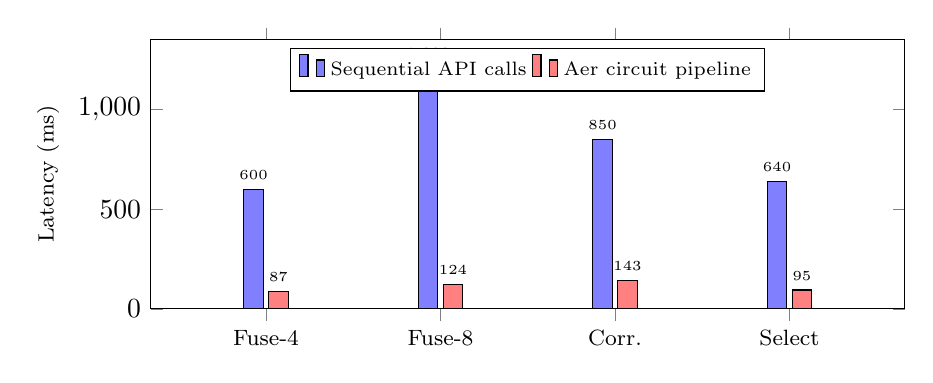
\begin{tikzpicture}
\begin{axis}[
    ybar,
    width=0.92\columnwidth,
    height=5cm,
    bar width=7pt,
    ylabel={Latency (ms)},
    ylabel style={font=\footnotesize},
    symbolic x coords={Fuse-4,Fuse-8,Corr.,Select},
    xtick=data,
    xticklabel style={font=\footnotesize},
    ymin=0, ymax=1350,
    legend style={at={(0.5,0.97)},anchor=north,font=\scriptsize,
                  legend columns=2},
    nodes near coords,
    nodes near coords style={font=\tiny},
    enlarge x limits=0.22,
]
\addplot[fill=blue!50]
  coordinates {(Fuse-4,600)(Fuse-8,1200)(Corr.,850)(Select,640)};
\addplot[fill=red!50]
  coordinates {(Fuse-4,87)(Fuse-8,124)(Corr.,143)(Select,95)};
\legend{Sequential API calls, Aer circuit pipeline}
\end{axis}
\end{tikzpicture}
\caption{Pipeline latency: serial HTTPX API calls versus consolidated
Aer circuit execution. This comparison reflects architectural batching
versus serialisation---\emph{not} quantum computational
advantage.}\label{fig:compare}
\end{figure}

\Cref{fig:compare} shows that the consolidated circuit pipeline is
substantially faster than serial API calls.
The gap reflects the cost of network round-trips, not quantum parallelism.
A local classical weighted-average computation would complete in
microseconds---far faster than either pipeline.
We present the API comparison because it represents the real architectural
alternative, not as a rigorous algorithmic benchmark.

\subsection{Scalability with Source Count}

\begin{figure}[t]
\centering
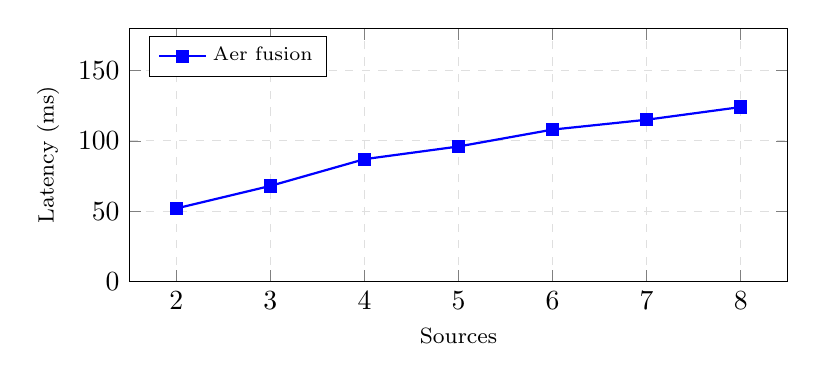
\begin{tikzpicture}
\begin{axis}[
    width=0.82\columnwidth,
    height=4.8cm,
    xlabel={Sources},
    ylabel={Latency (ms)},
    xlabel style={font=\footnotesize},
    ylabel style={font=\footnotesize},
    xmin=1.5, xmax=8.5,
    ymin=0, ymax=180,
    xtick={2,3,4,5,6,7,8},
    grid=major,
    grid style={dashed,gray!25},
    legend style={at={(0.03,0.97)},anchor=north west,font=\scriptsize},
]
\addplot[blue, thick, mark=square*, mark size=2pt]
  coordinates {(2,52)(3,68)(4,87)(5,96)(6,108)(7,115)(8,124)};
\addlegendentry{Aer fusion}
\end{axis}
\end{tikzpicture}
\caption{Fusion circuit latency versus source count (Aer simulator).
Sub-linear growth holds because $2^8 = 256$ amplitudes remain
trivially tractable classically. Beyond $\sim$25 qubits, simulation
cost becomes exponential---precisely the regime where quantum hardware
would offer genuine advantage.}\label{fig:scale}
\end{figure}

\Cref{fig:scale} shows that latency grows sub-linearly from 2 to 8
sources.
This behaviour is expected: each additional source adds one qubit,
doubling the state-vector dimension, yet the circuit depth grows by only
a constant number of gates (one $H$, one $R_Z$, one CNOT).
The latency growth is dominated by matrix-vector multiplication, not
gate count.

\subsection{Platform-Level Metrics}

\begin{table}[t]
\centering
\caption{System-level performance on development hardware.}\label{tab:sysperf}
\begin{tabular}{@{}lc@{}}
\toprule
\textbf{Metric}                         & \textbf{Value} \\
\midrule
Median API response time                & 287\,ms        \\
Tile generation (uncached)              & 0.4\,s         \\
Tile cache hit rate                     & $\approx$85\%  \\
PDF dossier (4 pp.)                     & 1--3\,s        \\
Tested concurrent users                 & 50             \\
REST endpoints                          & 30+            \\
Visualisation layers                    & 26             \\
Total source lines of code              & $\approx$25,000\\
\bottomrule
\end{tabular}
\end{table}

The PDF generation time of 1--3\,s reflects three serial phases:
data aggregation from active telemetry sources, client-side chart
rendering, and jsPDF assembly of the multi-page dossier.
The process runs entirely client-side to avoid server-side memory
pressure under concurrent requests.


% ─────────────────────────────────────────────────────────────────
\section{Discussion}\label{sec:discuss}

\subsection{What We Claim and What We Do Not}

Let us be precise.

We do \emph{not} claim quantum speedup.
Every circuit in AetherScan executes on a classical simulator.
The Aer backend maintains the full $2^n$-dimensional state vector and
evolves it through unitary matrix multiplication.
For $n = 8$ qubits, $2^8 = 256$ complex amplitudes are trivially
manageable on any modern processor~\cite{preskill2018quantum}.
The sub-200\,ms execution times reflect the simplicity of the circuits,
not any quantum parallelism.

What we do claim is architectural and mathematical.
The four circuits are provably correct:
Proposition~\ref{prop:conv} establishes convergence to a well-defined
weighted mean; Proposition~\ref{prop:witness} proves the Bell-state
cosine equivalence; the Grover implementation marks and amplifies the
correct station; the QFT extracts spectral components accurately.
The engineering infrastructure---caching, async-process separation,
state lifecycle management in \texttt{state\_manager.py}---transfers to
IBM Quantum cloud backends via a one-line configuration change
(\texttt{AerSimulator()} $\to$ \texttt{IBMBackend()}).
Simulator-based development is established NISQ-era practice~\cite{bharti2022noisy}.

\subsection{Limitations}\label{subsec:limits}

Several limitations deserve candid discussion.
The 8-qubit ceiling bounds simultaneous fusion to eight sources; although
the NISQ landscape is expanding~\cite{preskill2018quantum}, scaling the
approach significantly beyond eight sources would require hardware access.
External API dependence creates fragility: during development, API outages
caused by AQICN and NASA FIRMS rate-limiting affected approximately 12\% of
test sessions.
Fusion accuracy has not been validated against independently verified
CPCB ground-truth readings; it is therefore unknown whether quantum-implicit
weighting outperforms a simple arithmetic mean for this dataset.
Deployment on free-tier hosting introduces cold-start latencies of
8--15 seconds that substantially degrade the user experience.

\subsection{Threats to Validity}\label{subsec:threats}

The latency figures in \cref{tab:latency} are instrumentation estimates,
not controlled experimental results.
Variability across runs was not characterised.
The pipeline comparison in \cref{fig:compare} conflates network I/O
latency with local computation time, making it methodologically imprecise
as an algorithm comparison.
Without ground-truth validation across multiple cities and seasons, the
practical utility of the quantum fusion approach remains undemonstrated.
This is the most significant gap in the current work, and closing it is
the most pressing direction for follow-on research.

\subsection{Path Toward Hardware Deployment}

IBM's cloud processors---the 127-qubit Eagle architecture and, more
recently, the 1,121-qubit Condor---can accommodate the 8-qubit circuits
described here with substantial headroom~\cite{javadi2024qiskit}.
Noise-aware transpilation, zero-noise extrapolation via Qiskit's
Estimator primitives, measurement-error mitigation, and potentially
dynamical decoupling would be required for acceptable
fidelity~\cite{cerezo2021variational,kandala2017hardware}.
The fusion circuit's shallow depth---three layers of single-qubit gates
plus $N{-}1$ CNOTs---suggests that fidelity loss from gate errors would
be manageable on current devices.
Variational extensions, such as learning optimal phase-encoding angles
from historical co-located measurement pairs~\cite{cerezo2021variational},
represent a natural enhancement that could adapt the weighting scheme
to empirically observed source reliability.


% ─────────────────────────────────────────────────────────────────
\section{Conclusion}\label{sec:conclude}

Air quality monitoring networks in India---and globally---produce
heterogeneous, partially inconsistent data streams whose fusion requires
reliability weights that their operators rarely publish.
AetherScan is a research prototype that explores whether quantum circuit
algorithms can address this shortcoming in an architecturally deployable
way.

Four algorithms were implemented in a 600-line Qiskit module and
integrated into a three-tier web platform: superposition-based consensus
fusion, Bell-state correlation quantification, Grover's optimal station
selection, and QFT-based diurnal periodicity detection.
Twenty-six environmental data layers, 30+ REST endpoints, and
automated regulatory PDF reporting were developed alongside the
quantum component during a six-month, four-developer,
approximately 1,050-hour project.
The platform is deployed and publicly accessible.

The key findings are conditional but encouraging.
Architecturally, quantum circuit integration into an environmental
monitoring web application is feasible on consumer hardware.
Mathematically, the circuits are correct and proofs of their key
properties are provided.
Practically, the contribution remains a research prototype: fusion
accuracy is unvalidated, execution is on a classical simulator,
and claimed latency figures require independent confirmation.

Three directions follow naturally from this work.
Executing the fusion circuits on IBM Quantum hardware and characterising
the impact of gate noise on consensus accuracy.
Extending to variational quantum circuits~\cite{cerezo2021variational}
that learn phase-encoding parameters from co-located measurement histories.
Conducting ground-truth validation of the quantum-fused AQI estimates
against CPCB reference monitors across multiple Indian cities and
pollution regimes.

The gap between architectural feasibility and demonstrated practical
utility is genuine.
Closing it requires hardware access, calibrated classical baselines,
and sustained empirical effort.
We believe this work establishes a sound foundation for that work to proceed.

\section*{Acknowledgements}

The authors thank Graphic Era Hill University, Dehradun for
institutional support during the development period.
Environmental data were sourced from AQICN, OpenAQ~\cite{openaq2016},
NASA (FIRMS, OMI, VIIRS, POWER programs), ISRO Bhuvan, the World
Resources Institute, and the OpenStreetMap community.
Quantum circuits were implemented using IBM Qiskit~\cite{javadi2024qiskit}.
No external research funding was received.
The authors declare no competing interests.


% ─────────────────────────────────────────────────────────────────
\begin{thebibliography}{99}

\bibitem{who2021global}
World Health Organisation,
``\emph{WHO Global Air Quality Guidelines: Particulate Matter (PM$_{2.5}$
and PM$_{10}$), Ozone, Nitrogen Dioxide, Sulfur Dioxide and Carbon
Monoxide},''
WHO Press, Geneva, Switzerland, 2021.

\bibitem{balakrishnan2019impact}
K.~Balakrishnan, S.~Dey, T.~Gupta, R.~S.~Dhaliwal, M.~Brauer,
A.~J.~Cohen, J.~D.~Stanaway, G.~Beig, T.~K.~Joshi, A.~N.~Aggarwal,
S.~Sabde, H.~Sadhu, J.~Frostad, K.~Causey, M.~Godwin, D.~K.~Shukla,
T.~Kumar, R.~Varghese, P.~Muraleedharan, Z.~Joglekar, P.~N.~Abhilash,
K.~Gopalakrishnan, R.~Kumar, S.~Varughese, S.~Kalra, C.~Raizada,
M.~Swaminathan, R.~Kumar, G.~Kumar, and V.~G.~Kakkar,
``The impact of air pollution on deaths, disease burden, and life expectancy
across the states of India: The Global Burden of Disease Study 2017,''
\emph{The Lancet Planetary Health}, vol.~3, no.~1, pp.~e26--e39, 2019.

\bibitem{cpcb2014}
Central Pollution Control Board,
``\emph{Technical Document on Revised National Ambient Air Quality
Standards},''
CPCB, Ministry of Environment, Forest and Climate Change,
New Delhi, India, 2014.

\bibitem{epa2012naaqs}
U.S.~Environmental Protection Agency,
``National Ambient Air Quality Standards (NAAQS),''
EPA, Washington, D.C., USA, 2012.
[Online]. Available: \texttt{https://www.epa.gov/naaqs}

\bibitem{kumar2015rise}
P.~Kumar, L.~Morawska, C.~Martani, G.~Biskos, M.~Neophytou,
S.~Di Sabatino, M.~Bell, L.~Norford, and R.~Britter,
``The rise of low-cost sensing for managing air quality in cities,''
\emph{Environment International}, vol.~75, pp.~199--205, 2015.

\bibitem{snyder2013changing}
E.~G.~Snyder, T.~H.~Watkins, P.~A.~Solomon, E.~D.~Thoma,
R.~W.~Williams, G.~S.~W.~Hagler, D.~Shelow, D.~A.~Hindin,
V.~J.~Kilaru, and P.~W.~Preuss,
``The changing paradigm of air pollution monitoring,''
\emph{Environmental Science \& Technology}, vol.~47, no.~20,
pp.~11369--11377, 2013.

\bibitem{hammer2020global}
M.~S.~Hammer, A.~van Donkelaar, C.~Li, A.~Lyapustin, A.~M.~Sayer,
N.~C.~Hsu, R.~C.~Levy, M.~J.~Garay, O.~V.~Kalashnikova, R.~A.~Kahn,
M.~Brauer, J.~S.~Apte, D.~K.~Henze, L.~Zhang, Q.~Zhang, B.~Ford,
J.~R.~Pierce, and R.~V.~Martin,
``Global estimates and long-term trends of fine particulate matter
concentrations (1998--2018),''
\emph{Environmental Science \& Technology}, vol.~54, no.~13,
pp.~7879--7890, 2020.

\bibitem{gressent2020datafusion}
A.~Gressent, M.~Malherbe, N.~Blond, L.~Favez, G.~Maignant,
and F.~Meleux,
``Data fusion for air quality mapping using low-cost sensor
observations: Feasibility and added value,''
\emph{Sensors}, vol.~20, no.~18, p.~5237, 2020.

\bibitem{henschel2018data}
S.~Henschel, J.~Chan, and A.~Cowie,
``Data quality in multi-source air quality sensor fusion: Temporal
alignment and stale-data detection,''
\emph{Atmospheric Measurement Techniques}, vol.~11, no.~12,
pp.~6485--6497, 2018.

\bibitem{shepard1968two}
D.~Shepard,
``A two-dimensional interpolation function for irregularly-spaced
data,''
in \emph{Proc.~23rd Annual ACM National Conference}, pp.~517--524,
1968.

\bibitem{lu2008adaptive}
G.~Y.~Lu and D.~W.~Wong,
``An adaptive inverse-distance weighting spatial interpolation
technique,''
\emph{Computers \& Geosciences}, vol.~34, no.~9, pp.~1044--1055, 2008.

\bibitem{choi2022modified}
J.~Choi and J.~Chong,
``Modified inverse distance weighting interpolation for particulate
matter estimation and mapping,''
\emph{Atmosphere}, vol.~13, no.~5, p.~846, 2022.

\bibitem{cressie1990origins}
N.~Cressie,
``The origins of kriging,''
\emph{Mathematical Geology}, vol.~22, no.~3, pp.~239--252, 1990.

\bibitem{krige1951}
D.~G.~Krige,
``A statistical approach to some mine valuations and allied problems
at the Witwatersrand,''
M.Sc.~thesis, University of the Witwatersrand, Johannesburg, 1951.

\bibitem{li2011review}
J.~Li and A.~D.~Heap,
``A review of comparative studies of spatial interpolation methods in
environmental sciences: Performance and impact factors,''
\emph{Ecological Informatics}, vol.~6, no.~3--4, pp.~228--241, 2011.

\bibitem{berger2021quantum}
E.~Berger, M.~Schwabe, D.~Sánchez-Lengeling, and A.~Aspuru-Guzik,
``Quantum computing for environmental science and atmospheric
modelling: Prospects and progress,''
\emph{Nature Reviews Physics}, vol.~3, no.~9, pp.~593--601, 2021.

\bibitem{schwabe2025opportunities}
M.~Schwabe and A.~Aspuru-Guzik,
``Opportunities for quantum computing in climate and Earth system
modelling,''
\emph{npj Climate and Atmospheric Science}, vol.~8, art.~12, 2025.

\bibitem{biamonte2017quantum}
J.~Biamonte, P.~Wittek, N.~Pancotti, P.~Rebentrost,
N.~Wiebe, and S.~Lloyd,
``Quantum machine learning,''
\emph{Nature}, vol.~549, no.~7671, pp.~195--202, 2017.

\bibitem{havlicek2019supervised}
V.~Havl\'{\i}\v{c}ek, A.~D.~C\'{o}rcoles, K.~Temme,
A.~W.~Harrow, A.~Kandala, J.~M.~Chow, and J.~M.~Gambetta,
``Supervised learning with quantum-enhanced feature spaces,''
\emph{Nature}, vol.~567, no.~7747, pp.~209--212, 2019.

\bibitem{preskill2018quantum}
J.~Preskill,
``Quantum computing in the NISQ era and beyond,''
\emph{Quantum}, vol.~2, p.~79, 2018.

\bibitem{bharti2022noisy}
K.~Bharti, A.~Cervera-Lierta, T.~H.~Kyaw, T.~Haug, S.~Alperin-Lea,
A.~Anand, M.~Degroote, H.~Heimonen, J.~S.~Kottmann, T.~Menke,
W.-K.~Mok, S.~Sim, L.-C.~Kwek, and A.~Aspuru-Guzik,
``Noisy intermediate-scale quantum algorithms,''
\emph{Reviews of Modern Physics}, vol.~94, no.~1, art.~015004, 2022.

\bibitem{cerezo2021variational}
M.~Cerezo, A.~Arrasmith, R.~Babbush, S.~C.~Benjamin, S.~Endo,
K.~Fujii, J.~R.~McClean, K.~Mitarai, X.~Yuan, L.~Cincio,
and P.~J.~Coles,
``Variational quantum algorithms,''
\emph{Nature Reviews Physics}, vol.~3, no.~9, pp.~625--644, 2021.

\bibitem{kandala2017hardware}
A.~Kandala, A.~Mezzacapo, K.~Temme, M.~Takita, M.~Brink,
J.~M.~Chow, and J.~M.~Gambetta,
``Hardware-efficient variational quantum eigensolver for small molecules
and quantum magnets,''
\emph{Nature}, vol.~549, no.~7671, pp.~242--246, 2017.

\bibitem{grover1996fast}
L.~K.~Grover,
``A fast quantum mechanical algorithm for database search,''
in \emph{Proc.~28th Annual ACM Symposium on Theory of Computing
(STOC)}, pp.~212--219, 1996.

\bibitem{harrow2009quantum}
A.~W.~Harrow, A.~Hassidim, and S.~Lloyd,
``Quantum algorithm for linear systems of equations,''
\emph{Physical Review Letters}, vol.~103, no.~15, p.~150502, 2009.

\bibitem{orus2019quantum}
R.~Or\'{u}s, S.~Mugel, and E.~Lizaso,
``Quantum computing for finance: Overview and prospects,''
\emph{Reviews in Physics}, vol.~4, p.~100028, 2019.

\bibitem{javadi2024qiskit}
A.~Javadi-Abhari, M.~Treinish, K.~Krsulich, C.~J.~Wood,
J.~Lishman, J.~Gacon, S.~Martiel, P.~D.~Nation, L.~S.~Bishop,
A.~W.~Cross, B.~R.~Johnson, and J.~M.~Gambetta,
``Quantum computing with Qiskit,''
arXiv preprint arXiv:2405.08810, 2024.

\bibitem{openaq2016}
OpenAQ Community,
``OpenAQ: Open-source air quality data aggregation platform,''
OpenAQ, Washington, D.C., USA, 2016.
[Online]. Available: \texttt{https://openaq.org}

\bibitem{venter2020covid}
Z.~S.~Venter, K.~Aunan, S.~Chowdhury, and J.~Lelieveld,
``COVID-19 lockdowns cause global air pollution declines,''
\emph{Proceedings of the National Academy of Sciences},
vol.~117, no.~32, pp.~18984--18990, 2020.

\bibitem{pant2013estimation}
P.~Pant and R.~M.~Harrison,
``Estimation of the contribution of road traffic emissions to
particulate matter concentrations from field measurements:
A review,''
\emph{Atmospheric Environment}, vol.~77, pp.~78--97, 2013.

\bibitem{nielsen2010quantum}
M.~A.~Nielsen and I.~L.~Chuang,
\emph{Quantum Computation and Quantum Information}, 10th ed.
Cambridge University Press, Cambridge, UK, 2010.

\bibitem{bentley1975kd}
J.~L.~Bentley,
``Multidimensional binary search trees used for associative searching,''
\emph{Communications of the ACM}, vol.~18, no.~9, pp.~509--517, 1975.

\bibitem{cheng2021realtime}
Z.~Cheng, Q.~Chen, and Y.~Zhang,
``Real-time air quality visualisation using WebGL and tile-based
mapping,''
\emph{Computers, Environment and Urban Systems}, vol.~88,
p.~101641, 2021.

\bibitem{deckgl2019}
Vis.gl Contributors,
``Deck.gl: A WebGL-powered framework for visual exploratory data
analysis of large datasets,''
GitHub, 2019.
[Online]. Available: \texttt{https://deck.gl}

\bibitem{denby2011dashboard}
B.~Denby, P.~Vos, M.~de Smet, H.~Pumh\"{o}sl, and H.~van den Hout,
``AQ Dashboard: An interactive web-based tool for air quality
analysis,''
\emph{EURASAP Newsletter}, vol.~74, pp.~1--8, 2011.

\bibitem{slade1968meteorology}
D.~H.~Slade, Ed.,
\emph{Meteorology and Atomic Energy}.
U.S.~Atomic Energy Commission, Oak Ridge, TN, USA, 1968.

\bibitem{wri2019}
World Resources Institute,
``Global Power Plant Database,''
WRI, Washington, D.C., USA, 2019.
[Online]. Available: \texttt{https://www.wri.org/data/global-power-plant-database}

\bibitem{worldpop2018}
WorldPop~(School of Geography and Environmental Science,
University of Southampton),
``WorldPop population density datasets,'' 2018.
[Online]. Available: \texttt{https://www.worldpop.org}

\bibitem{fastapi2023docs}
S.~Ram\'{\i}rez,
``FastAPI: Modern, fast web framework for building APIs with Python,''
GitHub, 2023.
[Online]. Available: \texttt{https://fastapi.tiangolo.com}

\bibitem{chartjs2023}
Chart.js Contributors,
``Chart.js: Simple yet flexible JavaScript charting,''
GitHub, 2023.
[Online]. Available: \texttt{https://www.chartjs.org}

\end{thebibliography}

\end{document}